\section{Cloud Monitoring}\label{sec:cloud-monitoring}

\subsection{CloudWatch}\label{subsec:cloudwatch}
Provides metrics for every service in AWS. Some of these metrics are:

\begin{itemize}
    \item{\textbf{EC2 instances:} CPUUtilization, Status Checks, Network, etc.}
    \item{\textbf{EBS volumes:} Disk Read/Write, etc.}
    \item{\textbf{S3 buckets:} BucketSizeBytes, NumberOfObjects, etc.}
    \item{\textbf{Billing:} Total Estimated Charge, etc.}
\end{itemize}

\subsubsection{Alarms}
\textbf{Trigger notifications} for any metric.

\subsubsection{Logs}
Collects log and enable \textbf{real-time monitoring}\@.

\subsection{EventBridge}\label{subsec:eventbridge}
React to AWS events and connects this source to a destination (ex: lambda function, SNS topic).
The source can be 2 types:

\begin{itemize}
    \item{\textbf{Schedule:} Cron jobs.}
    \item{\textbf{Event Pattern:} Event rules (ex: IAM Root User Sign in Event).}
\end{itemize}

\begin{figure}[h]
    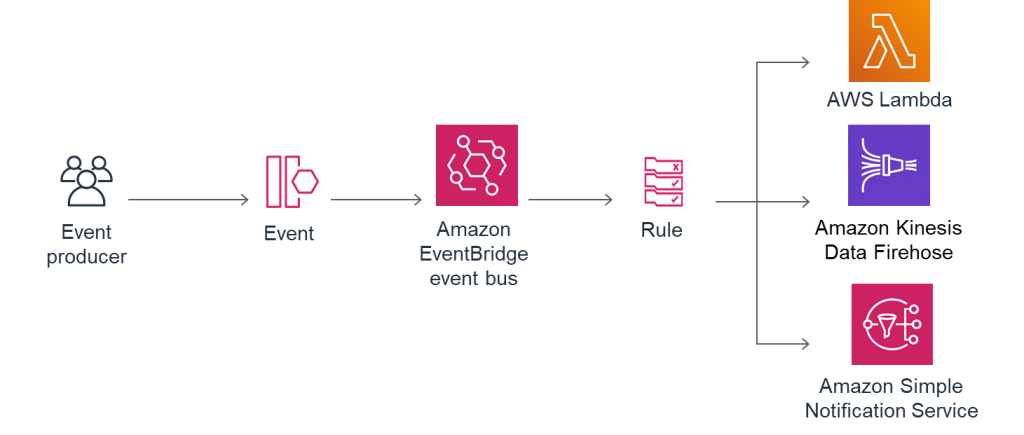
\includegraphics[scale=0.30]{cloud-monitoring/eventbridge}
    \centering
    \label{fig:eventbridge}
\end{figure}

\subsection{Cloudtrail}\label{subsec:cloudtrail}
Historical log of events/API calls made within an account (sdk, cli, console, iam user).
Cloudtrail provides governance, compliance and audit for AWS account.

\subsection{X-Ray}\label{subsec:x-ray}
Traces a path across all microservices and allows a visual analysis of the applications in order to
troubleshoot and debug any issue.

\subsection{CodeGuru}\label{subsec:codeguru}
ML powered service for \textbf{automated code review} and \textbf{application performance recommendations}.
It has 2 modes:

\begin{itemize}
    \item{\textbf{CodeGuru Review:} static code analysis.}
    \item{\textbf{CodeGuru Profiler:} recommendations during runtime.}
\end{itemize}

\subsection{Health Dashboard}\label{subsec:health-dashboard}

\subsubsection{Service health - History}
Shows all regions, \textbf{all services health}\@.

\subsubsection{Your account health dashboard}
\textbf{Provides alerts} and remediation guidance when AWS is experiencing \textbf{events that may impact you}\@.
Previously called AWS Personal Health Dashboard (PHD)\@.
